% =================================================================================================
% - this is the universal syntax of a LaTeX command: \command[options]{values}
% - in Ubuntu, installing texlive-full would provide all packages available
% =================================================================================================


% 1. set the document class
\documentclass[11pt]{article}  % article/book/letter/report/...



% 2. set the preamble
\usepackage{palatino}    % this is my favorite font
% \usepackage{tgpagella}   % this font looks similar but it doesn't apply to embedded code blocks

\usepackage{amsmath}     % for math equations
\usepackage{amssymb}     % font and typeface for math
\usepackage{mathpazo}    % font and typeface for math, this is my favorite

\usepackage{graphicx}    % for handling figures
\usepackage{subcaption}  % for handling subfigures
\usepackage{float}       % for setting the float (for strict figure positioning)

\usepackage{setspace}    % package that allows us to set the spacing for individual parts of the document

\usepackage{hyperref}    % for hyperlinks

\usepackage{listings}    % package that allows code in the document and offers source code highlighting
\usepackage{color}       % support colors in source code highlighting

\definecolor{darkgreen}{rgb}{0,0.6,0}  % define custom colors for later use in the document
\definecolor{gray}{rgb}{0.5,0.5,0.5}
\definecolor{mauve}{rgb}{0.58,0,0.82}

\usepackage{longtable}   % for multipage tables
\usepackage{booktabs}    % for prettier tables
\usepackage{multirow}    % enable a table cell to span multiple rows or multiple columns
\usepackage{siunitx}     % for numbers in a table column to be aligned at the decimal point, formatting unit and style...
\sisetup{                % specify how many decimal places should be displayed
  round-mode = places,   % round numbers
  round-precision = 2,   % to 2 decimal places
}

\usepackage[backend=bibtex,style=musuos]{biblatex}  % include biblatex, specify bibtex as the backend, and choose a style
\bibliography{latex}  % specify the bibliography database file, the .bib extension must be omitted


\title{LaTeX notebook}   % set up values for \maketitle for later use
\date{\today}            % or hard-code a date value
\author{Wentao Lu}

\setcounter{tocdepth}{2} % set the depth of table of contents(TOC)
                         % depth 1 will show only sections
                         % depth 2 will show sections and subsections
                         % depth 3 will show sections and subsections and subsubsections
                         % depth 4 = depth 3 + paragraphs
                         % depth 5 = depth 4 + subparagraphs

\lstset{  % this command predefines the default source code style settings all at once, here's a template from wikipedia
          % if we have many code blocks, each block can have its own formatting commands that override this setting
  language=c++,                             % the language of the code
  numbers=left,                             % where to put the line-numbers
  numberstyle=\tiny\color{gray},            % style of the line-numbers. \footnotesize\color{darkgray} is smaller
  stepnumber=1,                             % the step between two line-numbers. if set to 1, each line will be numbered
  numbersep=5pt,                            % how far the line-numbers are from the code
  backgroundcolor=\color{white},            % background color. \color[RGB]{245,245,244} is a little bit darker than white
  showspaces=false,                         % if set to true, underscores will be shown to indicate spaces
  showstringspaces=false,                   % if set to true, underscores will be shown to indicate spaces within strings
  showtabs=false,                           % if set to true, underscores will be shown to indicate tabs within strings
  frame=single,                             % add a frame around the code, if set to none, no frame will be displayed
  rulecolor=\color{black},                  % frame-color
  tabsize=4,                                % set default tabsize to 4 spaces
  captionpos=b,                             % set the caption-position to bottom
  breaklines=true,                          % set automatic line breaking
  breakatwhitespace=false,                  % set if automatic breaks should only happen at whitespace
  title=\lstname,                           % show the filename of the script included with \lstinputlisting
  keywordstyle=\color{blue},                % keyword style. \color[RGB]{40,40,255} is dark blue
  escapeinside={\%*}{*)},                   % if you want to add LaTeX within your code
  morekeywords={*,...},                     % if you want to add more keywords to the set
  basicstyle=\ttfamily\footnotesize,        % source code style
  commentstyle=\ttfamily\color{darkgreen},  % comment style. \it\color[RGB]{0,96,96} is italic dark green
  stringstyle=\ttfamily\color{mauve}        % string literal style. also try \rmfamily\slshape\color[RGB]{128,0,0}
}



% 3. structure the document

\begin{document}  % a \begin and \end statement defines an environment
                  % the "document" environment is always the topmost environment

  \pagenumbering{gobble}  % by convention, we suppress the page number in title and table of contents pages

  \maketitle  % create a titlepage defined in the preamble
  \newpage

  \doublespacing    % before generating TOC pages, set the spacing to double (double spacing TOC looks better)
  \tableofcontents  % create table of contents pages based on the section and subsection headings in the document
  \newpage          % to see the TOC displayed, we need to compile the .tex file twice

  \singlespacing    % after TOC pages are generated, reset the spacing back to single

  \pagenumbering{roman}   % pages should only be numbered after the titlepage and TOC. i,ii,iii,iv,v...
  \pagenumbering{Roman}   % I,II,III,IV,V...
  \pagenumbering{arabic}  % 1,2,3,4,5...


  % ------------------------------------ 1 -------------------------------------
  \section{Section 1: a sample hierarchical structure}
    Sections are numbered and will appear in the table of contents.

    \subsection{Subsection 1}
      Subsections are also numbered and will appear in the table of contents.

      \subsubsection{Subsubsection 1}
        And so forth...

        \paragraph{Paragraph 1}
        Paragraphs aren not numbered and won't show in the table of contents. Here this paragraph is given a name.\\

        By contrast, this paragraph is \textbf{not} given a name, it's an \textit{anonymous} paragraph. In practice, paragraphs do not need names unless we are writing math papers or technical documentation. It's also somewhat clumsy to start a new paragraph with \textit{\textbackslash paragraph\{\}} unless our sections and paragraphs are very deeply nested. More often, we can simply place a newline command \textit{\textbackslash newline} or \textit{\textbackslash \textbackslash} at the end of the previous paragraph.\\

        LaTeX will automatically indent the first line of each paragraph that doesn't immediately follow a section heading. Indeed, this format looks better.\\

        \noindent If you'd like to get rid of an indent anyway, use the \textit{\textbackslash noindent} command to start a paragraph, but this format does not look pretty and is not recommended since it breaks the default class structure.


  % ------------------------------------ 2 -------------------------------------
  \section{Math}
    There are two major modes of typesetting math in LaTeX one is embedding the math directly into your text by encapsulating your formula in dollar signs and the other is using a predefined math environment.

    % --------------------------------- 2.1 ---------------------------------
    \subsection{Using inline math - embed formulas in your text}
      If you need to typeset a single math symbol or formula, surround it with dollar signs: this formula $f(x) = x^2$ is an example.

    % --------------------------------- 2.2 ---------------------------------
    \subsection{The \textit{equation} and \textit{align} environment}
      The most useful math environments are the \textit{equation} environment for typesetting single equations and the \textit{align} environment for multiple equations and automatic alignment. These two environments also take care of equation numbers for us.\\

      The automatic numbering is a useful feature, but sometimes it's necessary to remove them for auxiliary calculations. LaTeX doesn't allow this by default, but we can include a package called \textit{amsmath} and add a * after the environment name. The asterisk (e.g. equation*, align*) only indicates, that I don't want the equations to be numbered. Note that it is not possible to enter two equations in a single \textit{equation} environment, it will result in a compilation error.

      \begin{equation}  % inside "document", multiple environments can be nested
        f(x) = x^2
      \end{equation}
      \begin{equation*}
        f(x) = x^3 + 3x + 13
      \end{equation*}

      The \textit{align} environment will align the equations at the ampersand \&. While it is possible to enter many equations in a single \textit{align} environment, different equations have to be separated by a linebreak \textbackslash \textbackslash. There is no alignment when using the simple \textit{equation} environment.

      \begin{align*}
        1 + 2 &= 3\\
        1 &= 3 - 2
      \end{align*}

    % --------------------------------- 2.3 ---------------------------------
    \subsection{Mathematical notation examples}
      All mathematical expressions have a unique command with unique syntax.

      \begin{align*}
        g(x) &= \frac{1}{x}\\              % \frac{u}{v} for fractions
        a(x) &= \int^a_b \frac{1}{3}x^3\\  % \int^a_b for integral symbol
        b(x) &= \frac{1}{\sqrt{x}}         % \sqrt{x} for square roots
      \end{align*}

      Use the \textit{matrix} environment to typeset matrices. \left[\begin{matrix}1 & 0\\0 & 1\end{matrix}\right]

      Scale parentheses with \textbackslash \textit{left}( \textbackslash \textit{right}) automatically. \left(\frac{1}{\sqrt{x}}\right)


  % ------------------------------------ 3 -------------------------------------
  \section{Images and figures}

    % --------------------------------- 3.1 ---------------------------------
    \subsection{Captioned images and figures}
      The \textit{figure} environment takes care of the numbering and positioning of the image within the document. All figures will be indexed automatically and tagged with successive numbers when using the \textit{figure} environment and the \textit{graphicx} package.\\

      At some point, you will notice that the figure doesn't necessarily show up in the exact place as you put your code in the .tex file. If your document contains a lot of text, it's possible that LaTeX will put the figure on the next page, or any other page where it finds sufficient space. To prevent this behavior, it's necessary to set the \textit{float} value for the \textit{figure} environment. Possible \textit{float} values are:

      \begin{itemize}
      	\item h (here) - same location
      	\item t (top) - top of page
      	\item b (bottom) - bottom of page
        \item p (page) - on an extra page
        \item ! (override) - will force the specified location
      \end{itemize}

      \begin{figure}[H]  % [h!] forces the figure to be shown here in the document, [H] is even stricter
        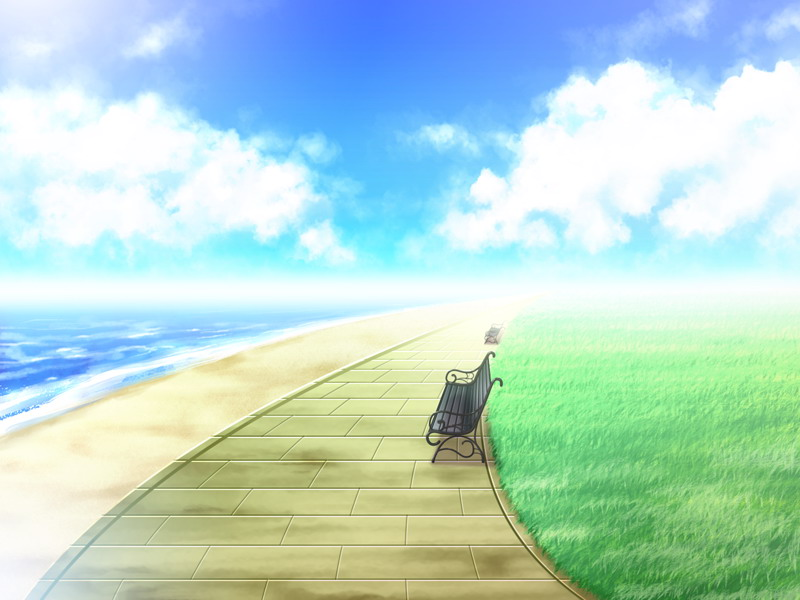
\includegraphics[width=\linewidth]{support/sample.JPG}  % the figure will be scaled to fit \linewidth
        \caption{This is a sample image.}  % caption of the figure is the text shown below the figure
        \label{f1}  % define a label for this figure, then later we can use \ref{f1} to reference it
      \end{figure}

    % --------------------------------- 3.2 ---------------------------------
    \subsection{Multiple images and subfigures}
      The \textit{subfigure} environment allows you to place multiple images at a certain location next to each other and the usage is pretty straightforward.\\

      First, we need to include the \textit{subcaption} package to the preamble. Next, we need to add multiple \textit{subfigure} environments within a \textit{figure} environment. Note that we must manually set the width of the image. If there are two images aligned next to each other, their widths should both be set to 0.4, but they still fill up the whole space. In such cases, we should always set the width to .1 less than we expect.

      \begin{figure}[h!]
        \centering
        \begin{subfigure}[h]{0.4\linewidth}  % must set the width of the image manually
          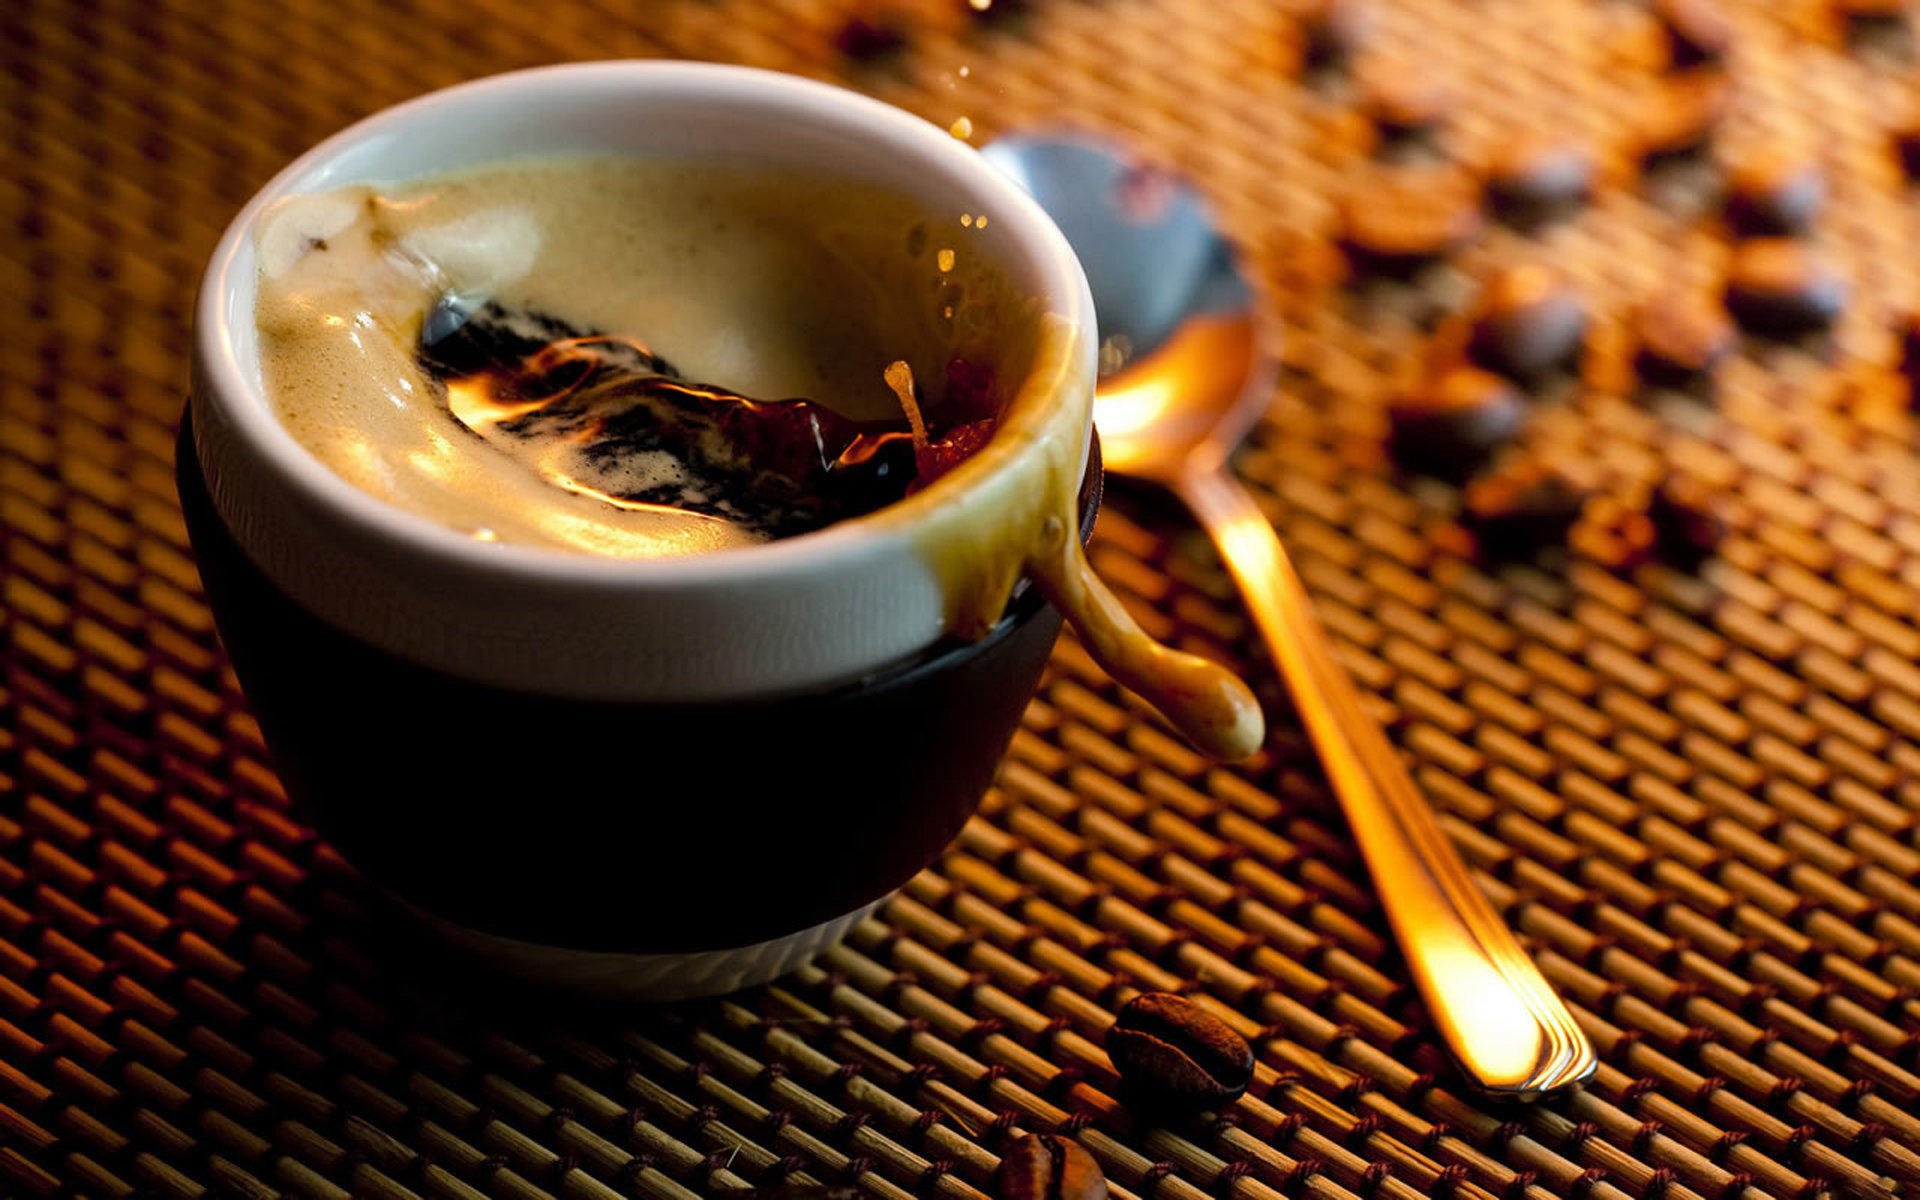
\includegraphics[width=\linewidth]{support/coffee.jpg}
          \caption{Coffee.}
        \end{subfigure}
        \begin{subfigure}[h]{0.4\linewidth}  % must set the width of the image manually
          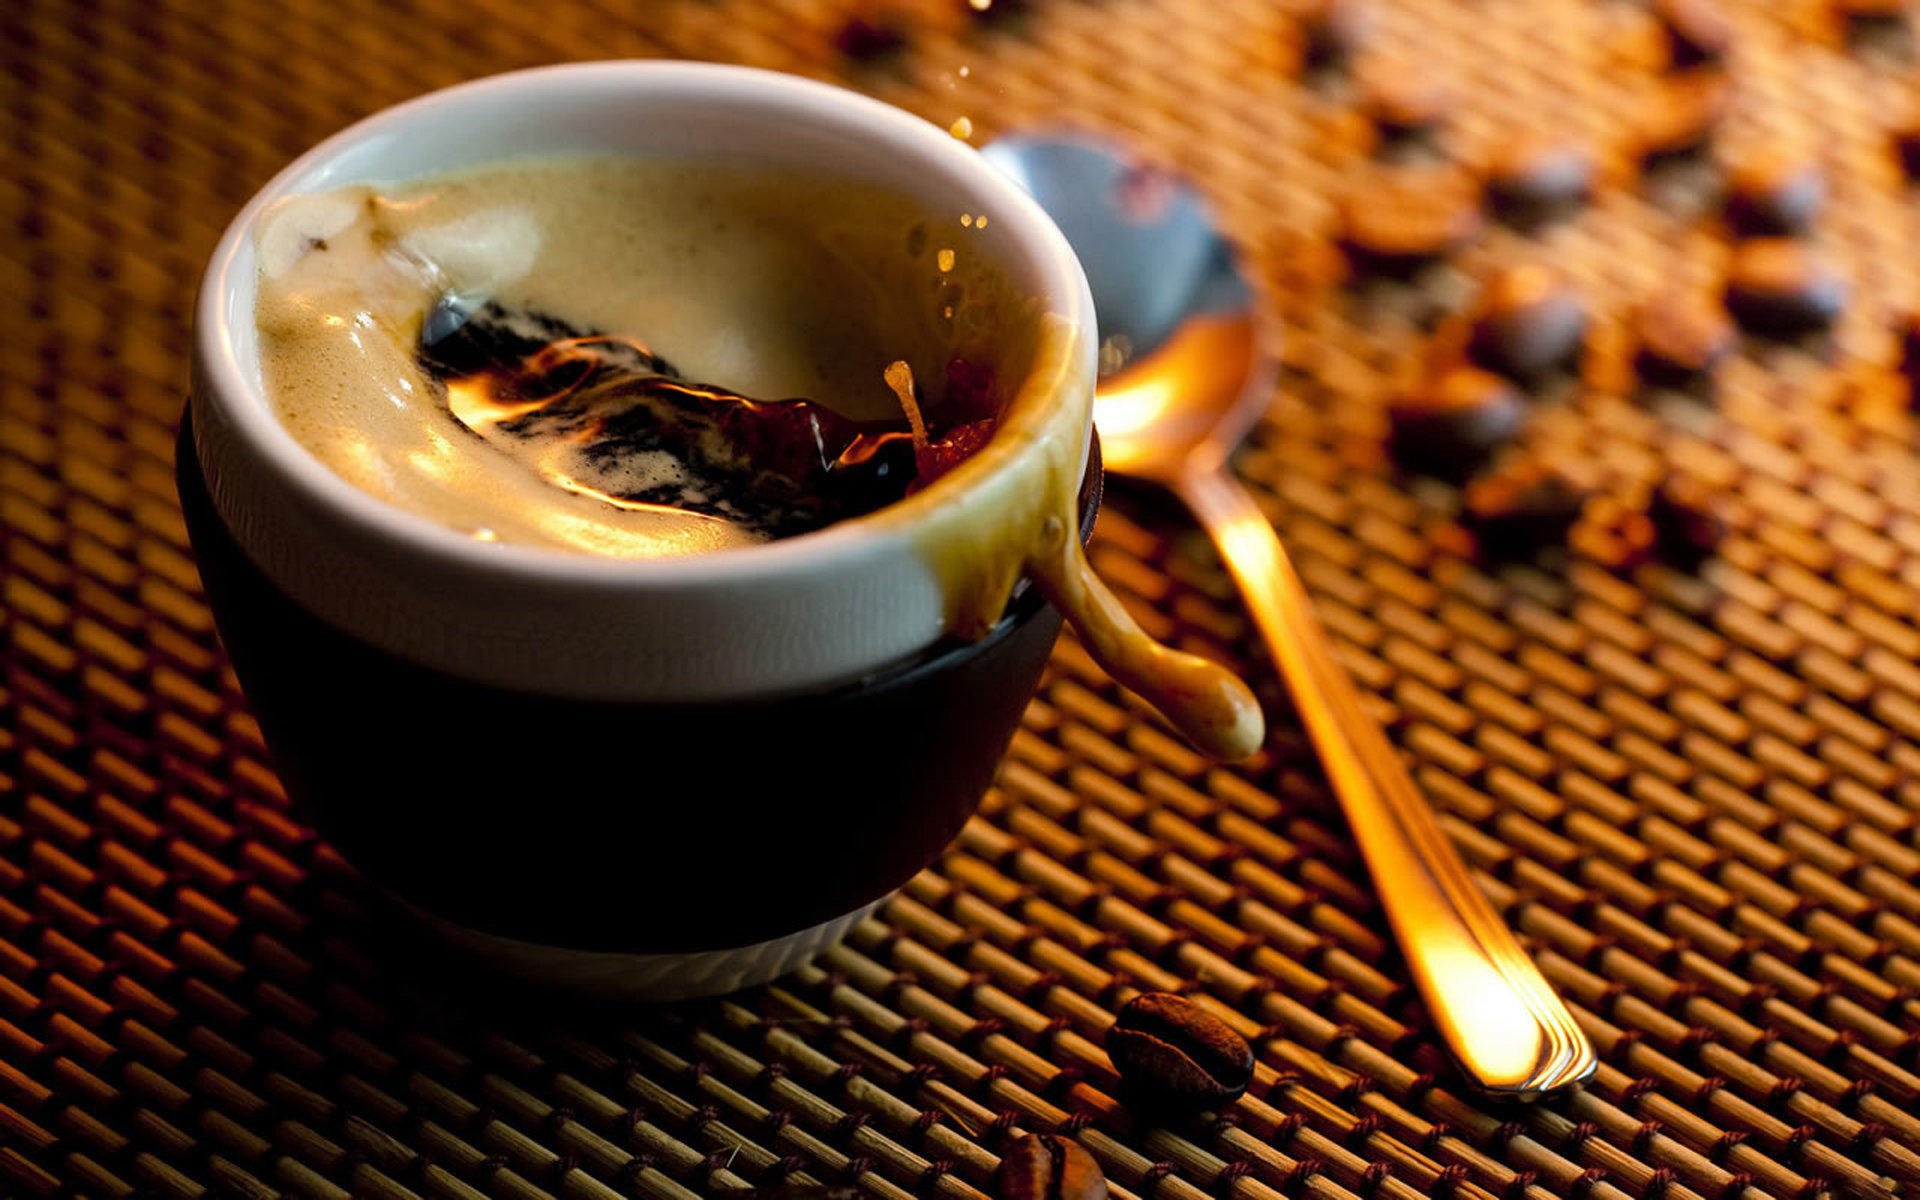
\includegraphics[width=\linewidth]{support/coffee.jpg}
          \caption{More coffee.}
        \end{subfigure}
        \caption{Two cups of coffee next to each other.}
        \label{f2}
      \end{figure}

      Likewise, if there are three images aligned next to each other, we should consecutively add three subfigures, each with a 0.2 \textit{\textbackslash linewidth} (1/3 - 0.1 = 0.2).

      \begin{figure}[h!]
        \centering
        \begin{subfigure}[h]{0.2\linewidth}
          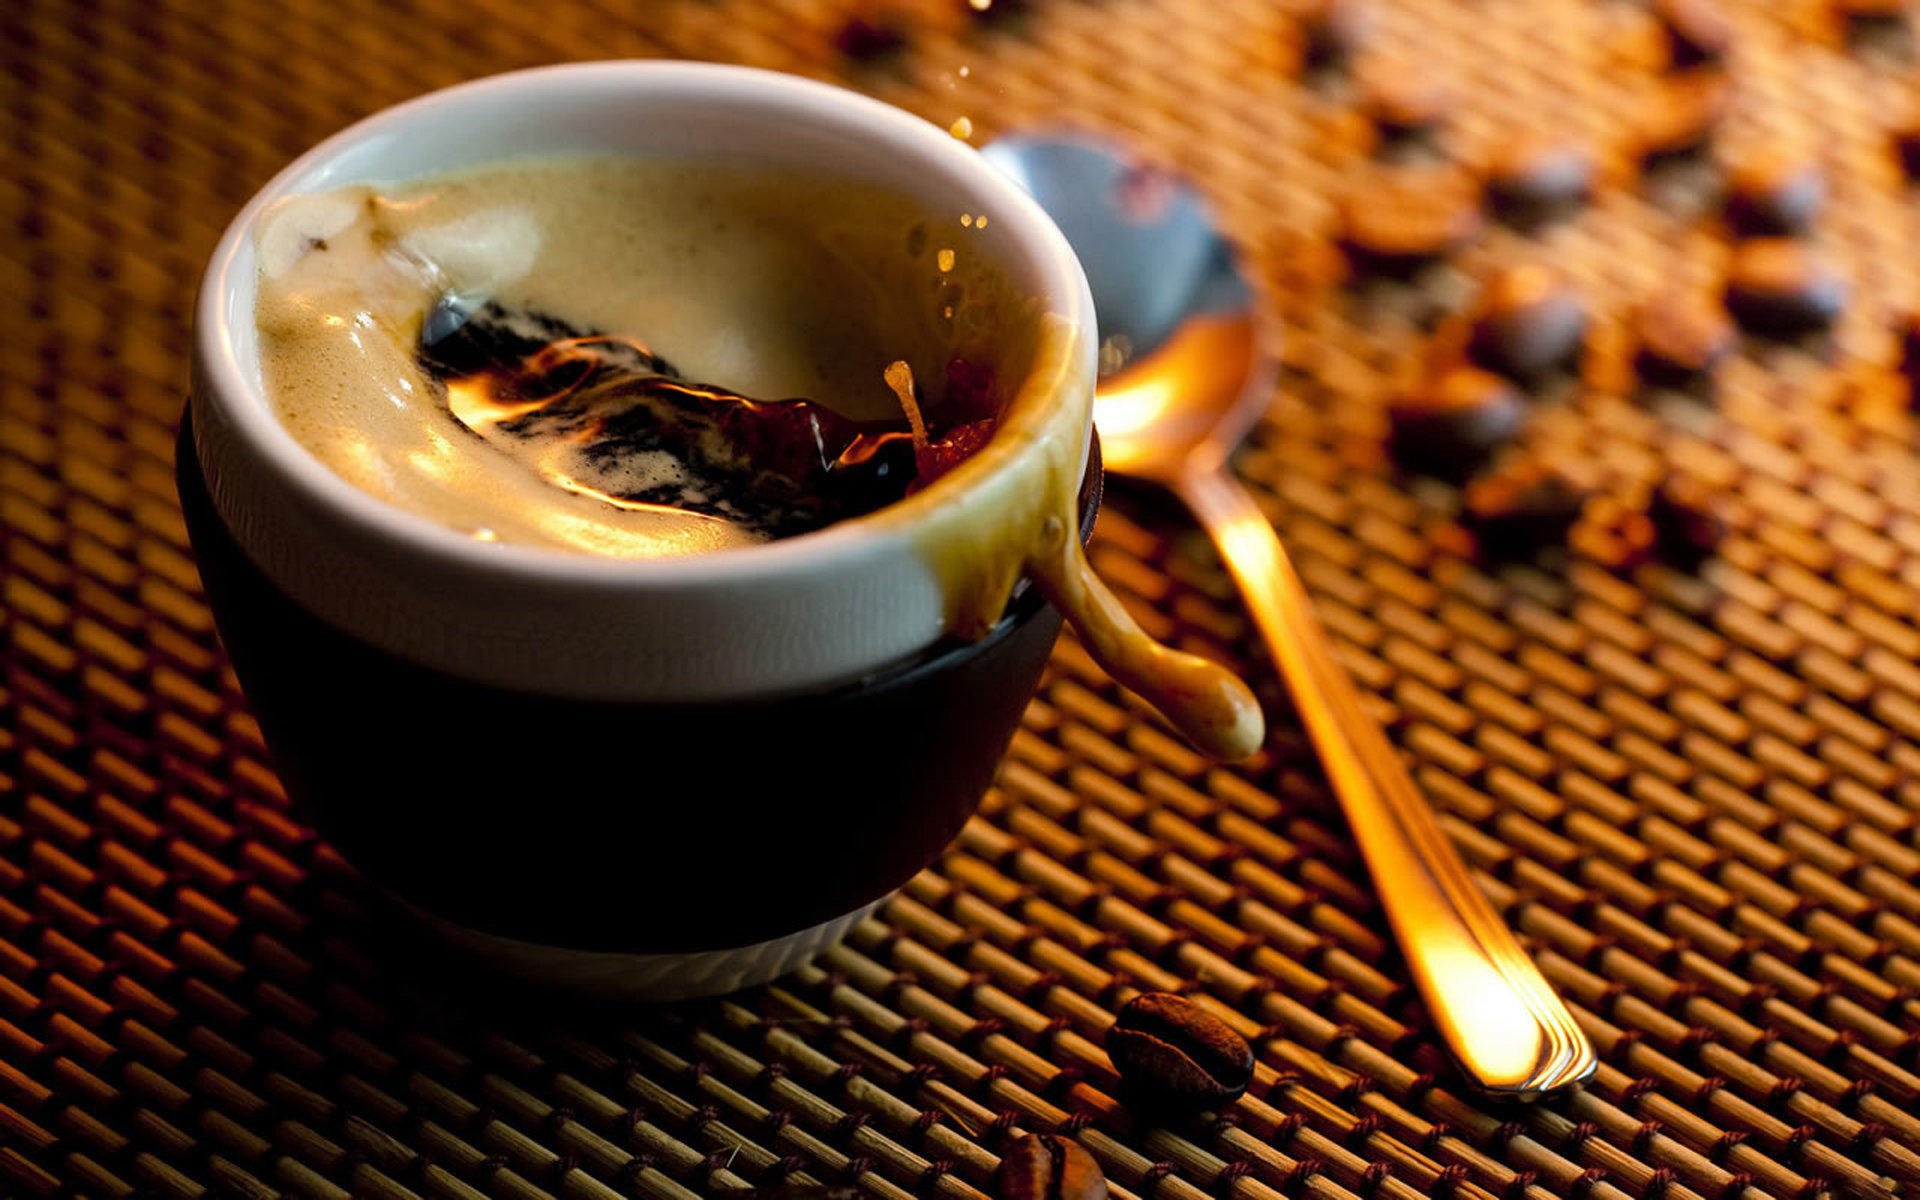
\includegraphics[width=\linewidth]{support/coffee.jpg}
          \caption{Coffee.}
        \end{subfigure}
        \begin{subfigure}[h]{0.2\linewidth}
          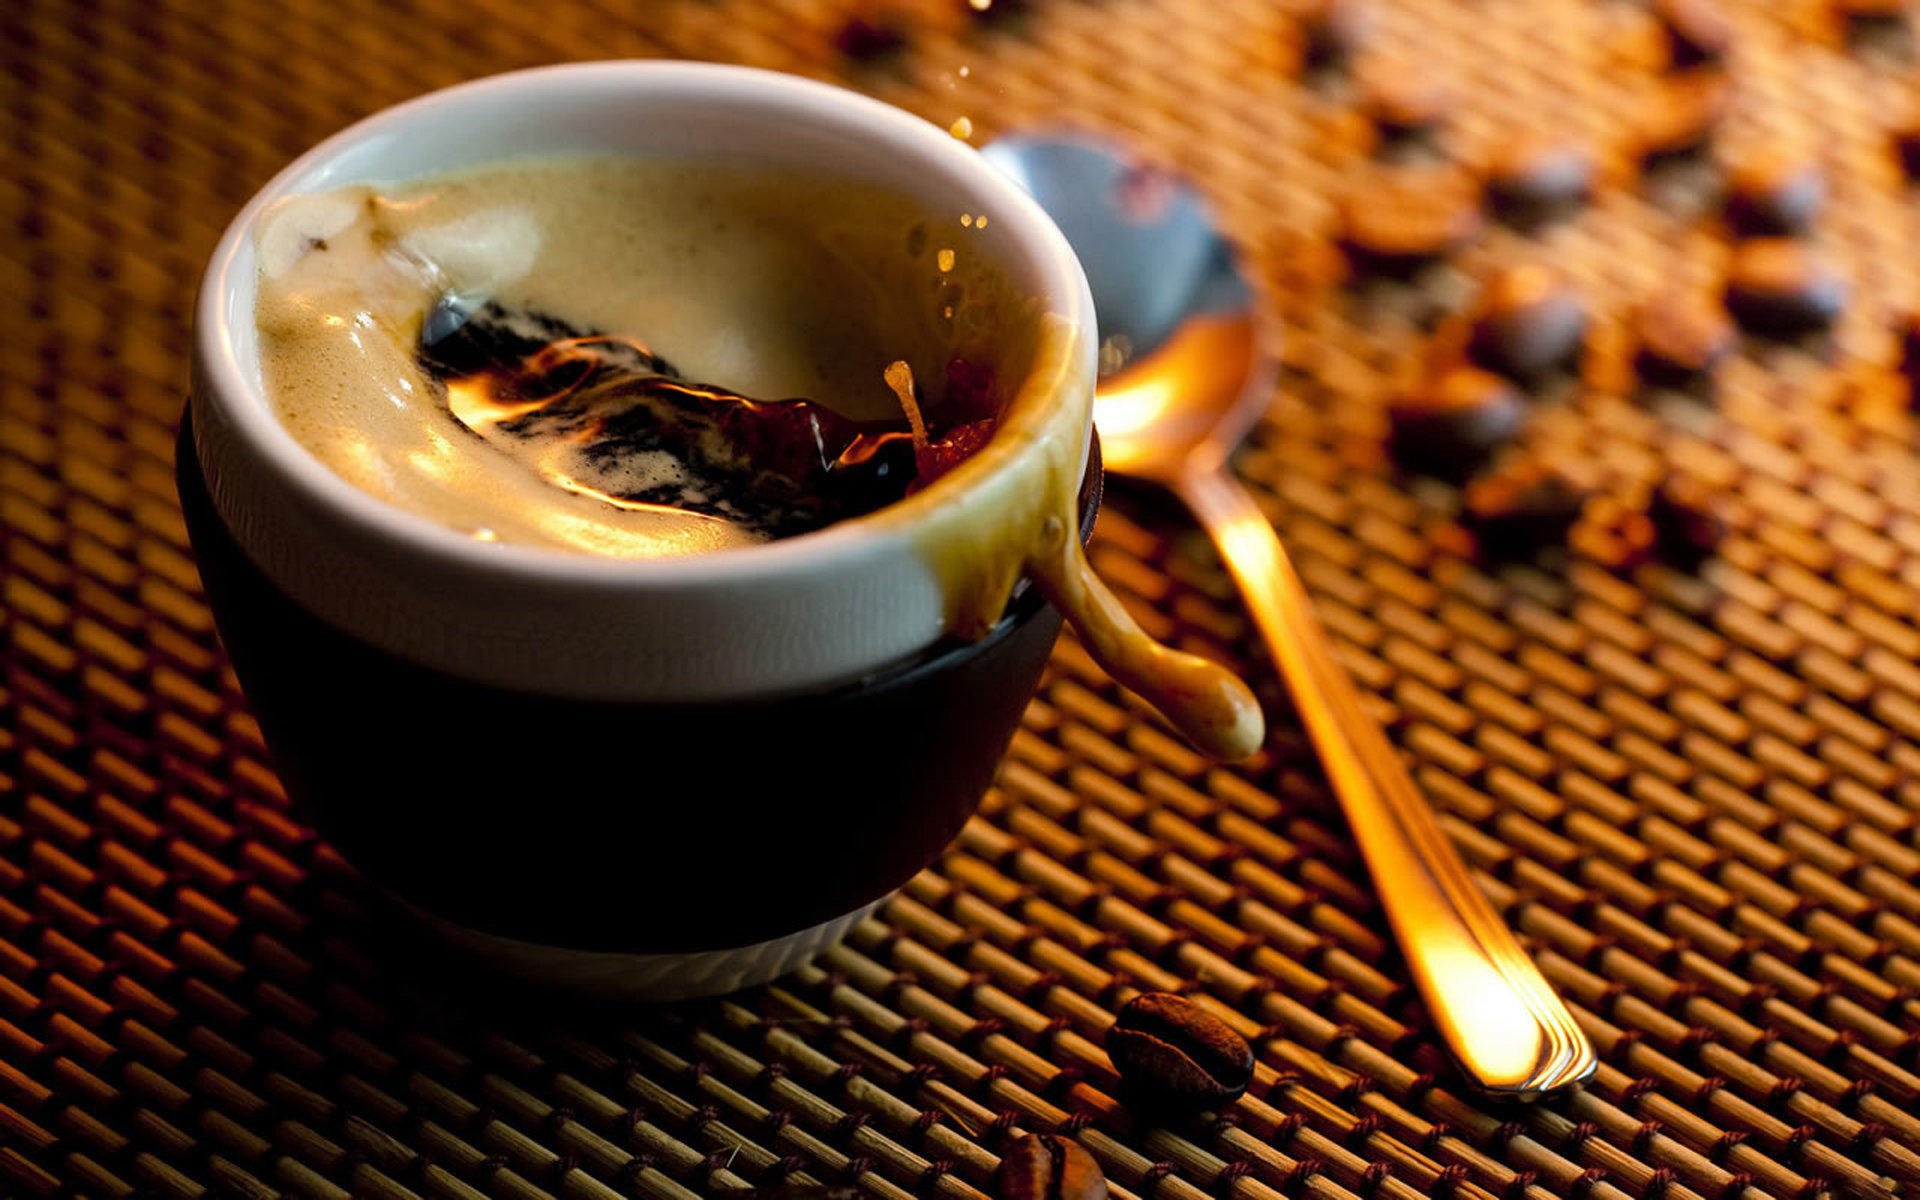
\includegraphics[width=\linewidth]{support/coffee.jpg}
          \caption{More coffee.}
        \end{subfigure}
        \begin{subfigure}[h]{0.2\linewidth}
          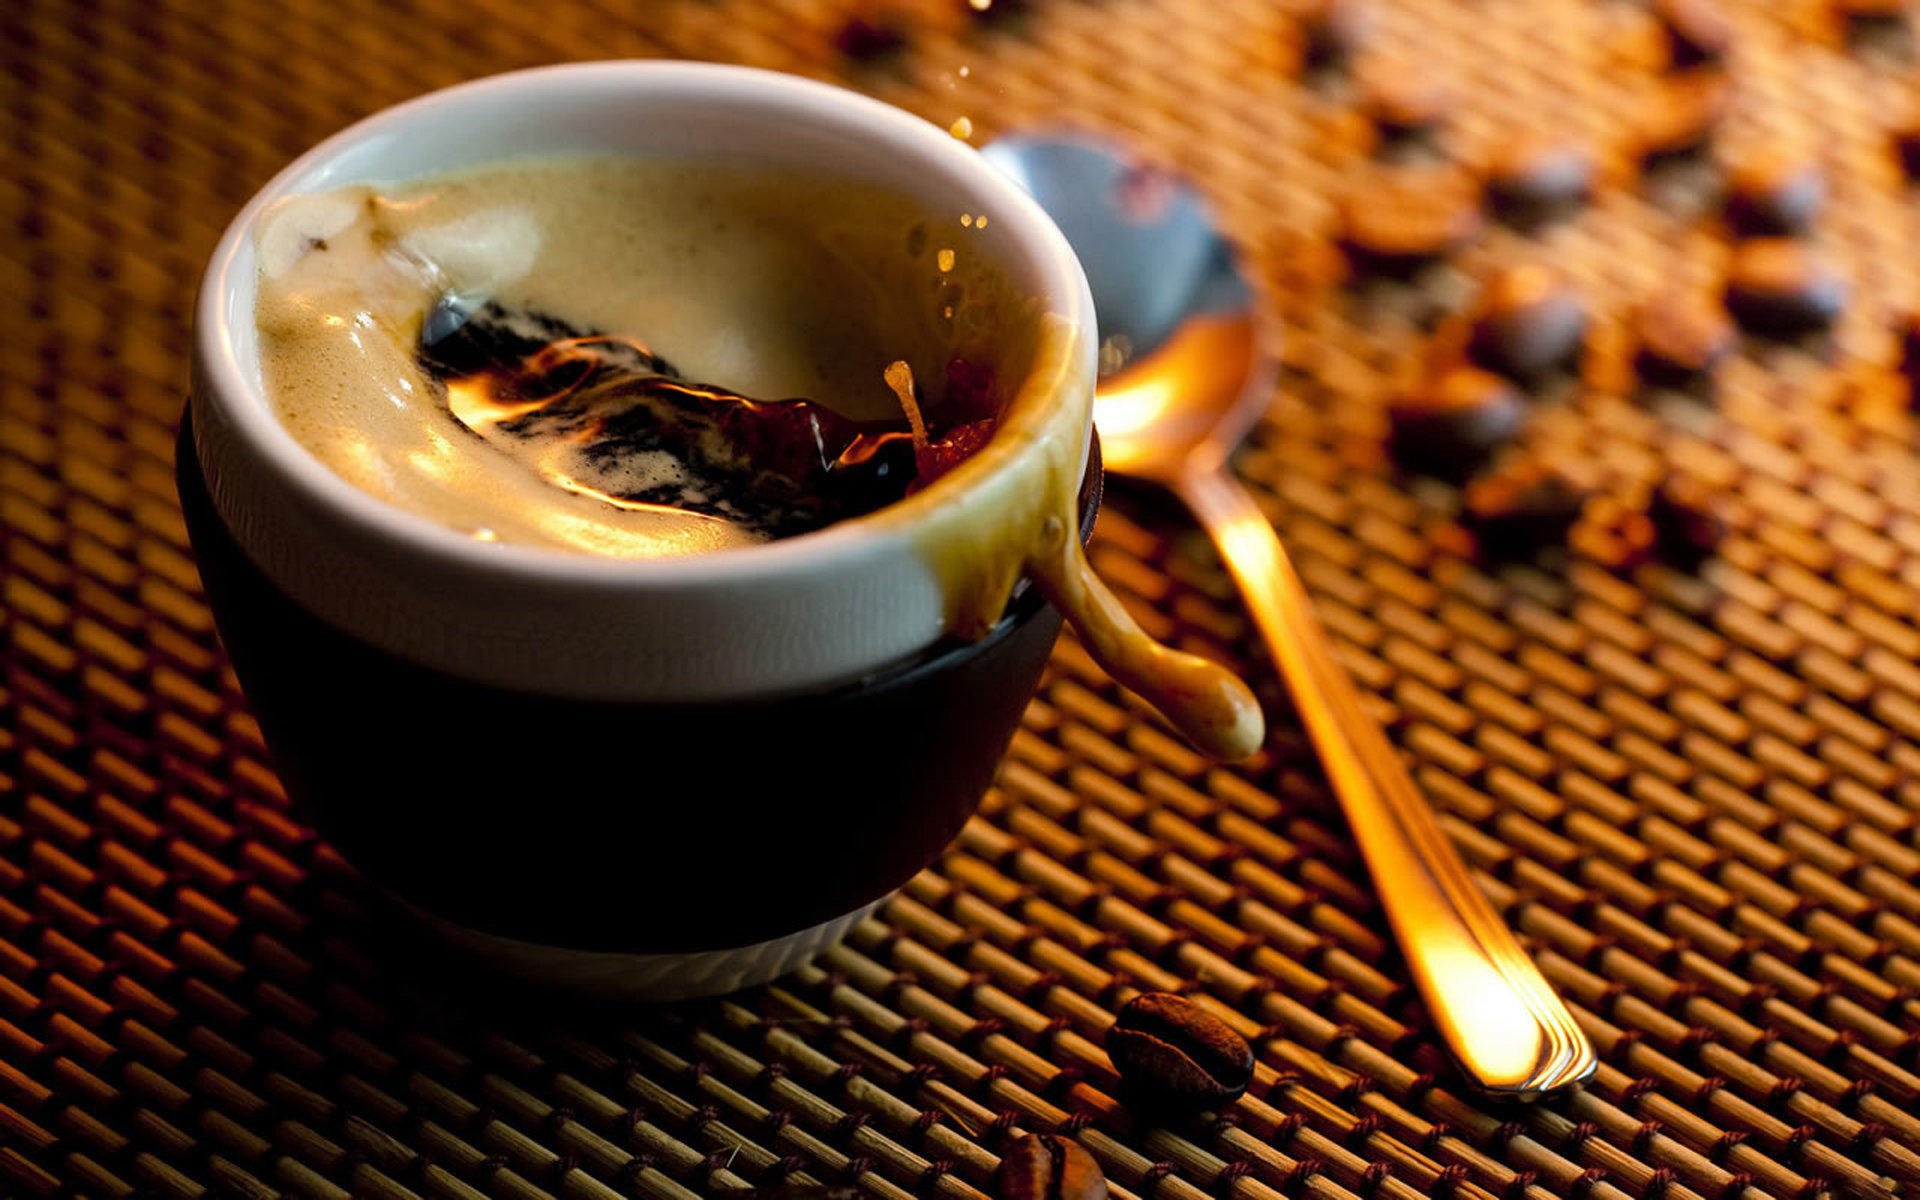
\includegraphics[width=\linewidth]{support/coffee.jpg}
          \caption{Tasty coffee.}
        \end{subfigure}
        \begin{subfigure}[h]{0.5\linewidth}  % 0.5 cannot fit on this row, so it goes to the next row
          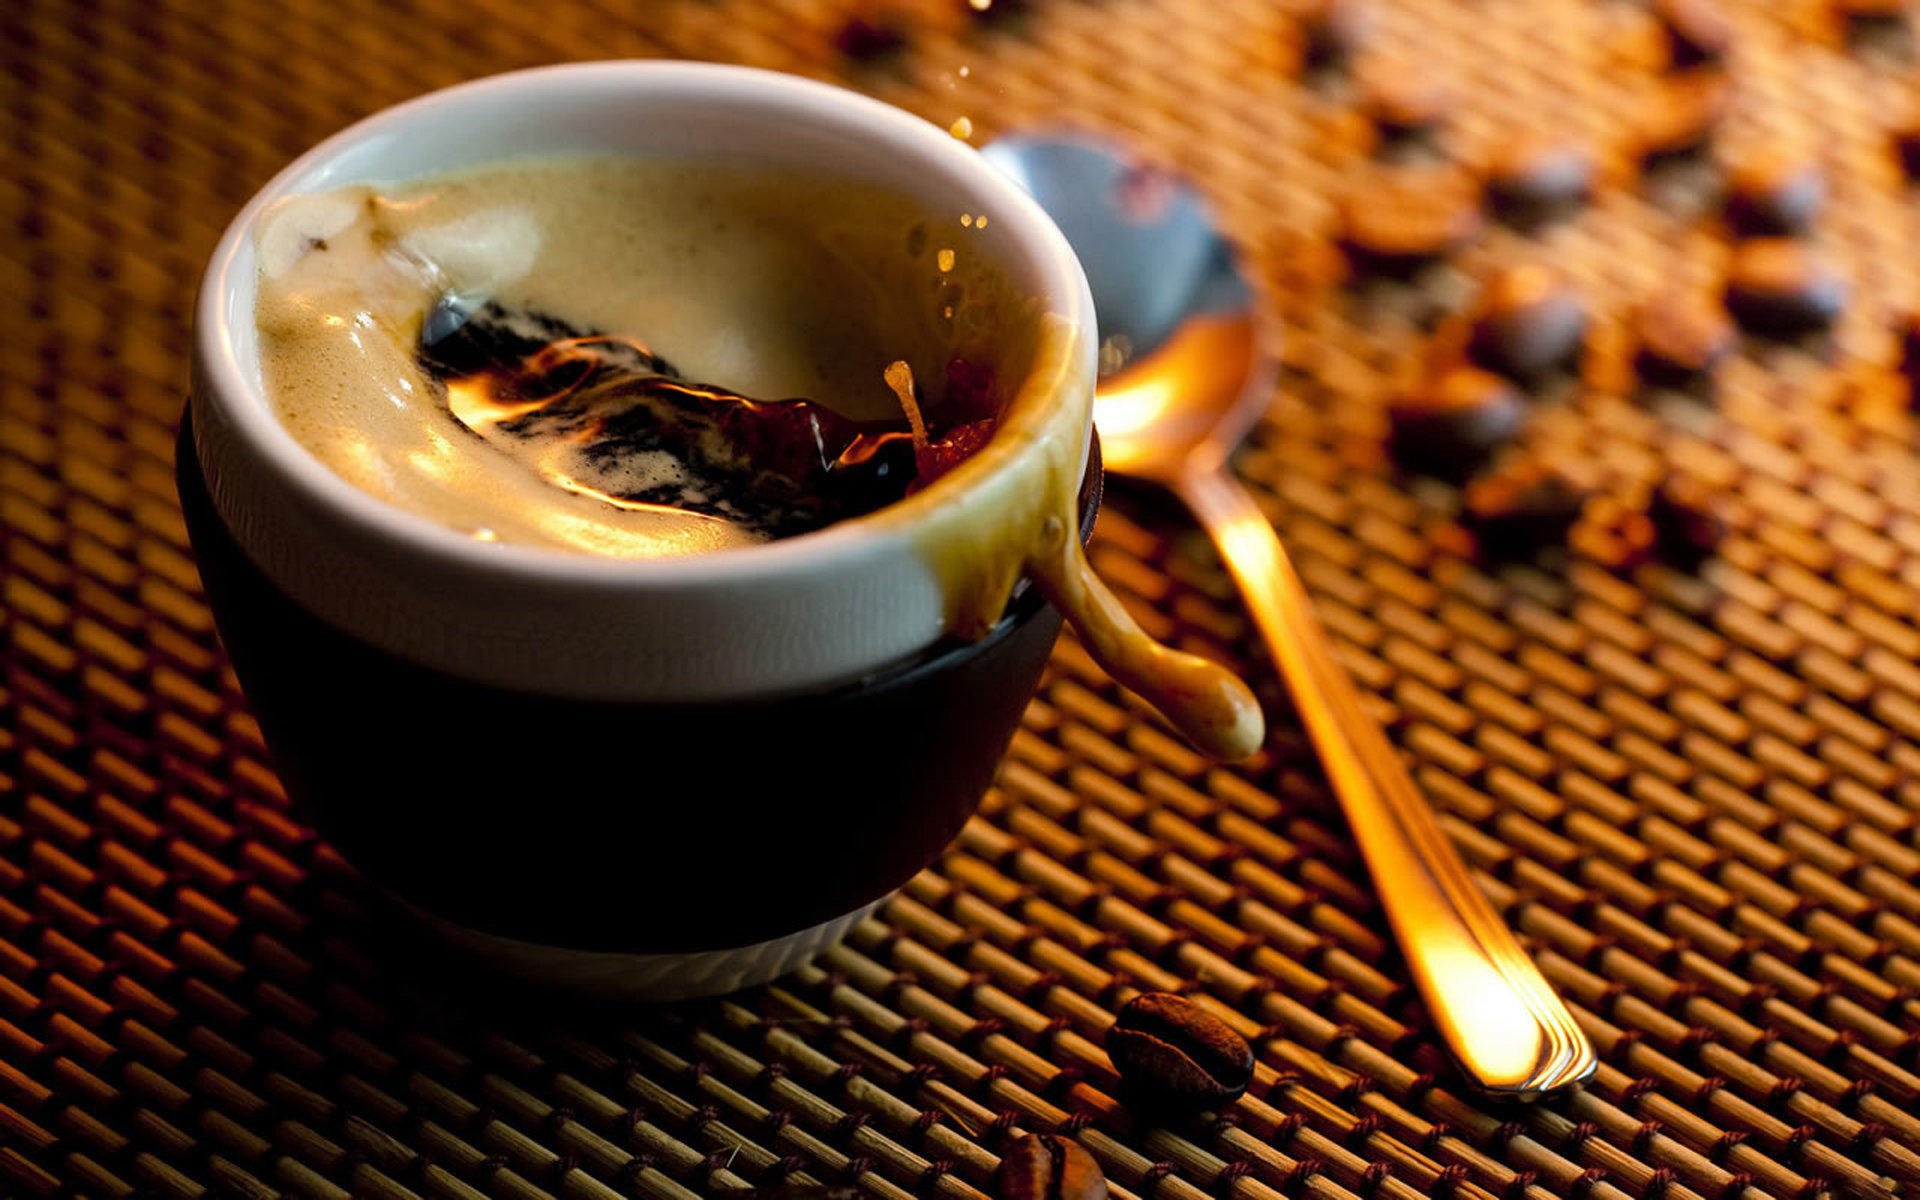
\includegraphics[width=\linewidth]{support/coffee.jpg}
          \caption{Too much coffee.}
        \end{subfigure}
        \caption{The same cup of coffee. Multiple times.}
        \label{f3}
      \end{figure}


  % ------------------------------------ 4 -------------------------------------
  \section{Bibliography}
    For simplicity, better compatibility and maintainability, it is recommended that we use \textit{bibtex} and \textit{biblatex} to create the bibliography. Briefly speaking, \textit{bibtex} is an external program that processes bibliography information in your .bib file, while \textit{biblatex} is a LaTeX package that formats citations and bibliographies. In other words, \textit{bibtex} reads input from our database (i.e. the .bib file) and transforms that .bib file into a .tex understandable one, and then, the LaTeX package \textit{biblatex} gives us access to use citing commands and display our bibliography in the final output .pdf file, this is how the pipeline works in general, despite that the real workflow is much more complicated.\\

    Alternatively, we also have some other choices such as \textit{biber} and \textit{natlib}, which are not in the scope of this notebook. For those who are interested, \href{https://tex.stackexchange.com/questions/25701/bibtex-vs-biber-and-biblatex-vs-natbib}{this post} contains a detailed introduction and comparison between all these tools.

    % --------------------------------- 4.1 ---------------------------------
    \subsection{Creating a .bib file}
      First we have to create a .bib file (bibliography database), which contains our bibliographic information. Here we have some examples.

      \lstinputlisting{latex.bib}

      Now let's closely look at the reference blocks in our .bib file and explain each field. There are three mandatory fields for all document classes. Be it an article, a book or an incollection, we must have the \textbf{author, year, title} fields. The string on the first line after \{ is a label that we use to refer to the item when we cite it. Inside the \textbf{author = \{\}} braces is the list of authors connected by "and", not by commas. Here commas are used to separate different parts of an author's name, where we should write in the form of "last name, first name". Inside the \textbf{title = \{\}} braces is the title of the reference, without quotation marks. For the \textbf{year} field, it must consist of only digits, and the braces around it can be omitted. All other fields are somewhat self-explanatory so we won't bother to cover them.\\

      For an article, we must also specify the \textbf{journal} field. For a book, the \textbf{publisher} field is also mandatory. Besides, the \textbf{author} field can also be replaced by an \textbf{editor} field, either of the two must be specified. For an incollection document class, fields \textbf{booktitle} and \textbf{publisher} are both mandatory. Likewise, \textbf{booktitle} is mandatory for inproceedings, \textbf{institution} is mandatory for techreport, and \textbf{note} is mandatory for unpublished document class.\\

      Inside each reference block structure, the order of the fields is unimportant. Our .bib file can contain references we don't cite. \textit{bibtex} will put in the list of references at the end of our paper only the ones that we cite.

    % --------------------------------- 4.2 ---------------------------------
    \subsection{Reading database and formatting references}
      Next, in the preamble we have to include the \textit{biblatex} package, specify \textit{bibtex} as the backend engine, choose a bibliographic formatting style, and then use the command \textit{\textbackslash bibliography} to tell LaTeX the location of our .bib file. Anywhere within the document, we can cite references using \textit{\textbackslash cite} and \textit{\textbackslash autocite}.\\

      For example, this is a citation \autocite{ab94} which is numbered and appears in the footnotes, and this is a citation whose full text description is directly embedded in the paragraph but does not appear in the footnotes: \cite{ahu61}.\\

      Here's another citation \autocite[32-35]{fk1988}  % we can specify page numbers in brackets as an option
      for which we have also specified the page numbers.\\

      Then, at the end of the document, we can use \textit{\textbackslash printbibliography} to create a separate reference page which will list all citations that have been cited.\\

      Finally, it's worth mentioning that there are many bibliography styles that we can use when we include the package \textit{biblatex}. \href{https://www.overleaf.com/learn/latex/Biblatex_bibliography_styles}{This post} has listed some of the most commonly used styles, with sample snapshots of how they look like. It is noteworthy that for different styles, the behaviors of the citing commands we mentioned above are also different. For some styles, the reference page could be empty, or the citation full text cannot be embedded. This is just a tutorial notebook, but when we write a formal paper, we should always stick to the style that is required by the university department.


  % ------------------------------------ 5 -------------------------------------
  \section{Footnotes}
    Footnotes are numbered automatically. For example, we can create a footnote of what coursera\footnote{\label{coursera}An American online learning platform founded by Stanford professors Andrew Ng and Daphne Koller that offers massive open online courses (MOOC), specializations, and degrees.} is, and later refer to it as footnote \ref{coursera}.


  % ------------------------------------ 6 -------------------------------------
  \section{Tables}
    Tables in LaTeX can be created through a combination of the \textit{table} environment and the \textit{tabular} environment. The \textit{table} environment part contains the caption and defines the float for our table, i.e. where in our document the table should be positioned and whether we want it to be displayed centered. The \textit{\textbackslash caption} and \textit{\textbackslash label} commands can be used in the same way as for pictures. The actual content of the table is contained within the \textit{tabular} environment.\\

    The \textit{tabular} environment uses ampersands \& to separate columns and newline symbol \textit{\textbackslash \textbackslash} to separate rows. A horizontal line can be added with the \textit{\textbackslash hline} command. Within a column, if we want to have numbers aligned at the decimal point, we can include the \textit{siunitx} package for this purpose, and setup the alignment using \textit{\textbackslash sisetup}.

    % --------------------------------- 6.1 ---------------------------------
    \subsection{A simple table}
      This is a simple table that works but is not very readable.

      \begin{table}[h!]
        \begin{center}
          \caption{A simple table.}
          \label{t1}
          \begin{tabular}{l|c|r}  % 1st column left-aligned, 2nd centered, 3rd right-aligned, with vertical lines in between
            \textbf{Value 1} & \textbf{Value 2} & \textbf{Value 3} \\  % 1st row
            $\alpha$         & $\beta$          & $\gamma$ \\          % 2nd row
            \hline  % row separator --------------------------------------------
            1                & 110.1            & a\\                  % 3rd row
            2                & 10.1             & b\\                  % 4th row
            3                & 23.113231        & c\\                  % 5th row
          \end{tabular}
        \end{center}
      \end{table}

      \begin{table}[h!]
        \begin{center}
          \caption{A simple table - numbers aligned.}
          \label{t2}
          \begin{tabular}{l|S|r}  % here "S" means: align the 2nd column as specified by \sisetup
            \textbf{Value 1} & \textbf{Value 2} & \textbf{Value 3} \\
            $\alpha$         & $\beta$          & $\gamma$ \\
            \hline
            1                & 110.1            & a\\
            2                & 10.1             & b\\
            3                & 23.113231        & c\\
          \end{tabular}
        \end{center}
      \end{table}

    % --------------------------------- 6.2 ---------------------------------
    \subsection{Cells spanning multiple rows or multiple columns}
      Sometimes it's necessary to make a row or column span several cells. For this purpose we can use the \textit{multirow} package. This package allows us to use the \textit{multirow} and \textit{multicolumn} environments, which make it easy to create a cell spanning multiple rows or columns.\\

      \begin{table}[h!]
        \begin{center}
          \caption{Multirow table.}
          \label{t3}
          \begin{tabular}{l|S|r}
            \textbf{Value 1}    & \textbf{Value 2} & \textbf{Value 3} \\
            $\alpha$            & $\beta$          & $\gamma$ \\
            \hline
            \multirow{2}{*}{12} & 1110.1           & a\\   % \multirow{number_of_rows}{width}{content}, "*" means automatic
                                & 10.1             & b\\   % the first column is omitted due to multirow
            \hline
            3                   & 23.113231        & c\\
            4                   & 25.113231        & d\\
          \end{tabular}
        \end{center}
      \end{table}

      If we want a cell to span multiple columns, we have to use the \textit{multicolumn} command. The usage differs a bit from \textit{multirow} command, since we also have to specify the alignment for our column. For example, in the row where we have a cell that spans two columns, there's only one column separator \& (instead of two for all other rows).\\

      \begin{table}[h!]
        \begin{center}
          \caption{Multicolumn table.}
          \label{t4}
          \begin{tabular}{l|S|r}
            \textbf{Value 1} & \textbf{Value 2} & \textbf{Value 3} \\
            $\alpha$         & $\beta$          & $\gamma$ \\
            \hline
            \multicolumn{2}{c|}{12}             & a\\  % combine two cells with alignment {c|} and content 12.
            \hline
            2                & 10.1             & b\\
            3                & 23.113231        & c\\
            4                & 25.113231        & d\\
          \end{tabular}
        \end{center}
      \end{table}

      Of course it's also possible to combine the two features, to make a cell spanning multiple rows and columns. To do this, we simply nest the \textit{multirow} command inside the \textit{multicolumn} command. The trick here is that, we have to add another \textit{multicolumn} statement for as many rows as we're combining.

      \begin{table}[h!]
        \begin{center}
          \caption{Multirow and -column table.}
          \label{t5}
          \begin{tabular}{l|S|r}
            \textbf{Value 1} & \textbf{Value 2}        & \textbf{Value 3} \\
            $\alpha$         & $\beta$                 & $\gamma$ \\
            \hline
            \multicolumn{2}{c|}{\multirow{2}{*}{1234}} & a\\  % \multirow serves as the content of \multicolumn
            \multicolumn{2}{c|}{}                      & b\\  % * empty \multicolumn statement serves as a placeholder
            \hline
            3                & 23.113231               & c\\
            4                & 25.113231               & d\\
          \end{tabular}
        \end{center}
      \end{table}

    % --------------------------------- 6.3 ---------------------------------
    \subsection{Prettier tables with booktabs}
      The \textit{booktabs} package provides much prettier horizontal separators. We can replace \textit{\textbackslash hline} with \textit{\textbackslash toprule}, \textit{\textbackslash midrule} and \textit{\textbackslash bottomrule}.

      \begin{table}[H]
        \begin{center}
          \caption{Table using booktabs.}
          \label{t6}
          \begin{tabular}{c|S|c}
            \toprule  % -----------------------------------------------
            \textbf{Value 1} & \textbf{Value 2} & \textbf{Value 3} \\
            $\alpha$         & $\beta$          & $\gamma$ \\
            \midrule  % -----------------------------------------------
            1                & 110.1            & a\\
            2                & 10.1             & b\\
            3                & 23.113231        & c\\
            \bottomrule  % --------------------------------------------
          \end{tabular}
        \end{center}
      \end{table}

    % --------------------------------- 6.4 ---------------------------------
    \subsection{Multipage tables}
      If you have a lot of rows in your table, you will notice that by default, the table will be cropped at the bottom of the page, which is certainly not what you want. The package \textit{longtable} provides a convenient way, to make tables span multiple pages. It's actually easier to use this package since the \textit{longtable} environment combines the previous \textit{table} and \textit{tabular} environment into a single environment. Using this environment, we create a table, that is automatically split between pages, if it has too many rows.

      \begin{longtable}[c]{c|S|c|c|c}  % \begin{longtable}[position_on_page]{alignment}
        \caption{Multipage table.}
        \label{t7}\\
        \toprule
        \textbf{Value 1} & \textbf{Value 2} & \textbf{Value 3} & \textbf{Value 4} & \textbf{Value 5} \\
        $\alpha$         & $\beta$          & $\gamma$         & $\epsilon$       & $\eta$           \\
        \midrule
        \endfirsthead    % end of the first header, which will be shown on the first page only

        % in between \endfirsthead and \endhead is the subsequent header
        \toprule
        \textbf{Value 6} & \textbf{Value 7} & \textbf{Value 8} & \textbf{Value 9} & \textbf{Value 0} \\
        $\delta$         & $\theta$         & $\lambda$        & $\kappa$         & $\psi$           \\
        \midrule

        \endhead         % end of the subsequent header, which will be shown on every page except the first page
        10               & 110.1            & a63              & apple            & orange \\
        29               & 10.1             & b73              & apple            & orange \\
        38               & 23.113231        & c65              & apple            & orange \\
        47               & 523.1            & a98              & apple            & orange \\
        56               & 120.12           & b15              & apple            & orange \\
        65               & 3.72             & c35              & apple            & orange \\
        74               & 46.18            & a90              & apple            & orange \\
        83               & 14.0             & b34              & apple            & orange \\
        92               & 9.135            & c72              & apple            & orange \\
        01               & 532.24           & a84              & apple            & orange \\
        10               & 110.1            & a56              & apple            & orange \\
        29               & 10.1             & b38              & apple            & orange \\
        38               & 23.113231        & c93              & apple            & orange \\
        47               & 523.1            & a54              & apple            & orange \\
        56               & 120.12           & b66              & apple            & orange \\
        65               & 3.72             & c86              & apple            & orange \\
        74               & 46.18            & a33              & apple            & orange \\
        83               & 14.0             & b26              & apple            & orange \\
        92               & 9.135            & c18              & apple            & orange \\
        01               & 532.24           & a27              & apple            & orange \\
        10               & 110.1            & a58              & apple            & orange \\
        29               & 10.1             & b88              & apple            & orange \\
        38               & 23.113231        & c94              & apple            & orange \\
        47               & 523.1            & a56              & apple            & orange \\
        56               & 120.12           & b00              & apple            & orange \\
        \bottomrule
      \end{longtable}

    % --------------------------------- 6.5 ---------------------------------
    \subsection{Generating tables from .csv files}
      When writing papers, it is sometimes necessary to present a large amount of data in tables. Writing such tables by hand is very time-consuming and error-prone. To avoid this, we can simply import the data directly from .csv (comma-separated value) files. For this purpose, we can use the \textit{pgfplotstable} package. Similarly, there's also a package called \textit{pgfplots} for automatic plot generation from .csv files. However, this notebook will not cover them here because such cases are rare. It's not useful to learn about the redundant features since we already have better tools such as Python for tackling with these tasks. The point is, for whatever task we have, wisely choose the most appropriate toolbox.


  % ------------------------------------ 7 -------------------------------------
  \section{Source code}
    The required packages and settings have already been setup in the preamble part, and the comments should be self-explanatory. To actually insert source code in the document, there are mainly two ways. One way is to directly copy and paste source code into the \textit{lstlisting} environment, but indentation could be troublesome since it will not ignore the indentation and spaces in the .tex file. As an alternative, it's preferable to use the \textit{\textbackslash lstinputlisting} command, which is able to read in a source code script file and outputs it to the .pdf, without messing up with our .tex file.\\

    \begin{lstlisting}[language=python]
      # indentation from the .tex file not ignored
      # when we directly copy and paste code
      @functools.singledispatch
      def show(obj):
          print(obj, type(obj), "obj")
    \end{lstlisting}

    \lstinputlisting{support/HelloWorld.cpp}  % \lstlinputlisting{filename}


  % ------------------------------------ 8 -------------------------------------
  \section{Hyperlinks}
    We can use the \textit{hyperref} package which allows us to set links with a description as well as add bare urls to the document. After the hyperlink is inserted, if there's a colored box shown around the word. Don't worry, this box is not going to show up in our printed document, but only if we view it on the computer.\\

    This is my homepage: \href{https://github.com/neo-mashiro}{neo-mashiro}.\\

    A bare URL without an description: \url{https://github.com/neo-mashiro}.\\

    My email address is: \href{mailto:neo-mashiro@hotmail.com}{neo-mashiro@hotmail.com}.


  % ------------------------------------ 9 -------------------------------------
  \section{Lists}
    Unordered lists use the \textit{itemize} environment.

    \begin{itemize}
      \item One
      \item Two
      \item Three
    \end{itemize}

    \noindent Ordered lists use the \textit{enumerate} environment.

    \begin{enumerate}
      \item One
      \item Two
      \item Three
    \end{enumerate}

    \noindent Nested lists are the products of nested list environments.

    \begin{enumerate}
      \item One
      \begin{enumerate}
      	\item Two
        \item Three
      \end{enumerate}
      \item Four
    \end{enumerate}

    \noindent It's easy to change the numbering scheme or the bullets of a list.

    \begin{itemize}
      \item[--] Dash
      \item[$-$] Dash
      \item[$\ast$] Asterisk
    \end{itemize}


  % ------------------------------------ appendix ------------------------------------
  \newpage
  \begin{appendix}  % after all sections, before references, is the appendix
    \listoffigures  % compile twice to generate the lists, same as TOC
    \listoftables   % compile twice to generate the lists, same as TOC
  \end{appendix}


  % ----------------------------------- references -----------------------------------
  \newpage
  \printbibliography

\end{document}
